\documentclass[12pt]{article}

\usepackage{amssymb}
\usepackage{amsmath}
\usepackage{bm}
\usepackage{color}
\usepackage{float}
\usepackage{graphicx}
\usepackage{mathtools}
\usepackage[none]{hyphenat}
\usepackage{indentfirst}
\usepackage[labelfont=bf]{caption}
\usepackage[left=2.5cm,right=2.5cm, top=2.5cm,bottom=2.5cm]{geometry}
\usepackage{tcolorbox}
\usepackage{lineno}
\usepackage{setspace}
\DeclarePairedDelimiter\ceil{\lceil}{\rceil}

\usepackage[authoryear]{natbib}
\usepackage{hyperref}
\usepackage{yhmath}
\usepackage{accents}

\usepackage{dsfont}
\usepackage{mathtools}
\usepackage{soul}

\overfullrule 5pt

\doublespacing

\usepackage{lipsum}

%\usepackage{adjustbox}
\usepackage{lscape}
\usepackage{afterpage}

\makeatletter
\renewcommand{\maketitle}{\bgroup\setlength{\parindent}{0pt}
\begin{flushleft}
\textbf{\@title}

  \@author
\end{flushleft}\egroup
}
\makeatother

\begin{document}

\linenumbers

\title{A Bayesian Model of the DNA Barcode Gap}

\author{Jarrett D. Phillips$^{1, 2*}$ (ORCID: 0000-0001-8390-386X), ... (others?)  \\
\textit{$^1$School of Computer Science, University of Guelph, Guelph, ON., Canada, N1G2W1} \\ \textit{$^2$Department of Integrative Biology, University of Guelph, Guelph, ON., Canada, N1G2W1} }

\date{}

\maketitle

\vspace{2mm}

\noindent \textbf{*Corresponding Author}: Jarrett D. Phillips$^{1}$

\noindent \textbf{Email Address}: jphill01@uoguelph.ca

\noindent \textbf{Running Title}: Bayesian inference for DNA barcode gap estimation

\newpage

\begin{abstract}

A simple statistical model of the DNA barcode gap is outlined. Specifically, \\ accuracy of recently introduced nonparametric metrics, inspired by coalescent theory, to characterize the extent of proportional overlap/separation in maximum and minimum pairwise genetic distances within and among species, respectively, is explored in both frequentist and Bayesian contexts. The empirical cumulative distribution function (ECDF) is utilized to estimate probabilities associated with positively skewed extreme tail distribution quantiles bounded on the closed unit interval [0, 1] based on a \\ straightforward binomial distance overlap count. Using R and Stan, the proposed maximum likelihood estimators and Bayesian model are demonstrated on cytochrome $b$ (CYTB) gene sequences from two \textit{Agabus} diving beetle species exhibiting limits in the extent of representative taxonomic sampling. Large-sample theory and MCMC simulations show much uncertainty in parameter estimates, particularly when specimen sample sizes for target species are small. Findings highlight the promise of the Bayesian approach using a conjugate beta prior for reliable posterior uncertainty estimation when available data are sparse. Obtained results can shed light on foundational and applied research questions concerning DNA-based specimen identification and species delineation for studies in evolutionary biology and ecology, as well as biodiversity conservation and management, of wide-ranging taxa.

\end{abstract}

\textbf{Keywords}: Bayesian/frequentist inference, DNA barcoding, intraspecific genetic \\ distance, interspecific genetic distance, specimen identification, species discovery

\vspace{2mm}

\section{Introduction}

The routine use of DNA sequences to support broad evolutionary hypotheses and \\ questions concerning demographic processes, like gene flow and speciation, is now ubiquitous. Since the late 1980s, mitochondrial DNA (mtDNA) has been employed to produce a \\ distinctive and measurable pattern of genetic polymorphism in diverse and \\ spatially-distributed  taxonomic lineages such as birds, fishes, insects, and arachnids, among other extensively studied groups \citep{avise1987intraspecific}. The application of genomic data to applied fields like biodiversity forensics, conservation, and management for the molecular identification of unknown  specimen samples came later (\textit{e.g.}, Forensically Informative \\ Nucleotide Sequencing (FINS); \citet{bartlett1992fins}). Since its inception over 20 years ago, DNA barcoding \citep{hebert2003biological, hebert2003barcoding} built significantly on earlier work and has emerged as a robust method of specimen identification and species discovery across myriad multicellular eukaryotes which have been sequenced at easily obtained short, standardized gene regions like the cytochrome $c$ oxidase subunit I (5'-COI) mitochondrial locus for animals. 

The success of the single-locus approach, particularly for regulatory and forensic \\ applications, depends crucially on two important factors: (1) the availability of high-quality specimen records found in public reference sequence databases such as the Barcode of Life Data Systems (BOLD; http://www.barcodinglife.org) \citep{ratnasingham2007bold} and GenBank (https://www.ncbi.nlm.nih.gov/genbank/), and (2) the establishment of a DNA barcode gap --- the notion that the maximum genetic distance observed within species is much smaller than the minimum degree of marker variation found among species \citep{meyer2005dna, meier2008use}. Early work has demonstrated that the presence of a DNA barcode gap hinges strongly on extant levels of species haplotype diversity gauged from comprehensive specimen sampling at wide geographic and ecological scales \citep{bergsten2012effect, candek2015dna}. Despite this, many taxonomic groups lack adequate separation in their pairwise intraspecific and interspecific genetic distances due to varying rates of evolution in both genes and taxa \citep{pentinsaari2016molecular}. Furthermore, it has been well demonstrated that the presence of a DNA barcode gap becomes less certain with increasing spatial scale of sampling since interspecific distances increase, while intraspecific distances shrink as more closely-related species are sampled \citep{phillips2022lack}. This can pose problems in cases of rare species or monotypic taxa, for instance \citep{ahrens2016rarity}.  As a result, rapid matching of unknown samples to expertly-validated references can be compromised, leading to cases of false positives (taxon oversplitting) and false negatives (excessive lumping of taxa) due to incomplete lineage sorting, interspecies \\ hybridization, genome introgression, species synonymy, cryptic species diversity, and \\ misidentifications \citep{hubert2015dna, phillips2022lack}.

Recent work has argued that DNA barcoding, in its current form, is lacking in statistical rigor, as most studies rely strongly on heuristic distance-based measures to infer taxonomic identity. Of these studies, few report measures of uncertainty, such as standard errors (SEs) and confidence intervals (CIs), around estimates of intraspecific and interspecific  variation (\textit{e.g.}, \citet{wiemers2007does}), calling into question the existence of a true species' DNA barcode gap \citep{candek2015dna, phillips2022lack}. To support this idea, novel nonparametric locus- and species-specific metrics based on the multispecies coalescent (MSC) were recently outlined by \citet{phillips2024measure}. The coalescent \citep{kingman1982coalescent, kingman1982genealogy} encompasses a backwards continuous-time stochastic Markov process of allelic sampling within natural, neutrally-evolving, species populations towards the most recent common ancestor (MRCA). Although the coalescent sampling process plays a foundational role in evolutionary and population genetics theory due to its inherent simplicity and flexibility, it has been both under-utilized and under-appreciated as a key player within DNA barcoding \citep{hubert2015dna, stoeckle2014dna, phillips2022lack}. Previously proposed MSC algorithmic approaches (of which there are too many to exhaustively list here), generally assume a strict molecular clock and a simplified model of DNA sequence evolution across closely-related taxa, from which an estimated species phylogeny may be constructed (\textit{e.g.}, with or without use of a guide tree) (\textit{e.g.}, \citet{rannala2003bayes, rannala2017efficient, yang2010bayesian, yang2014unguided, yang2017bayesian}). Even taxon delimation methods designed for single loci, such as the Generalized Mixed Yule Coalescent (GMYC) \citep{pons2006sequence, fujisawa2013delimiting} and Poisson Tree Processes (PTP) \citep{kapli2017multirate, zhang2013general}, which have seen much use in DNA barcoding initiatives, have their flaws. Optimal performance of these methods relies heavily on careful parameter selection (\textit{e.g.}, prior specification of branching rates in ultrametric trees) within third party software like BEAST \citep{bouckaert2019beast}, among other concerns \citep{fonseca2021gmyc}. In contrast, \citeauthor{phillips2024measure}'s (\citeyear{phillips2024measure}) approach is tree-free and does not require judicious parameter setting. Therefore, the method is extremely efficient and fast to run. 

The DNA barcode gap statistics have been shown to hold strong promise for reliable DNA barcode gap assessment when applied to predatory \textit{Agabus} (Coleoptera: Dytiscidae) diving beetles  \citep{phillips2024measure}. Despite their ease of sampling and well-established taxonomy, this group possesses few morphologically-distinct taxonomic characters that readily facilitate their assignment to the species level \citep{bergsten2012effect}. Further, the proposed metrics indicate that sister species pairs from this taxon are often difficult to distinguish on the basis of their DNA barcode sequences \citep{phillips2024measure}. Using sequence data from three mitochondrial cytochrome markers (5'-COI, 3'-COI, and cytochrome $b$ (CYTB)) obtained from BOLD and GenBank, results highlight that DNA barcoding has been a one-sided argument. \citeauthor{phillips2024measure}'s (\citeyear{phillips2024measure}) findings point to the need to balance both the sufficient collection of specimens, as well as the extensive sampling of species. Not surprisingly, DNA barcode libraries are biased toward the latter effort \citep{phillips2022lack}. 

The estimators from \citet{phillips2024measure} represent a clear improvement over simple, yet arbitrary, distance heuristics such as the 2\% rule noted by \citet{hebert2003biological} and the 10$\times$ rule \citep{hebert2004identification} that form the basis of single-locus species delimitation tools like Automatic Barcode Gap Discovery (ABGD) \citep{puillandre2011abgd}, Assemble Species by Automatic Partitioning (ASAP) \citep{puillandre2021asap}, and the Barcode Index Number (BIN) framework \citep{ratnasingham2013bin}. The 2\% rule asserts that DNA barcodes differing by at least 2\% at sequenced genomic regions should be expected to originate from different biological species, whereas the 10$\times$ rule suggests that sequences displaying 10 times more genetic variation among species than within taxa is evidence for a distinct evolutionary origin. However, the lack of adoption of an explicit, universally agreed upon, species concept that readily governs lineage formation and proliferation necessary to establish rigorous taxon definitions for successful delimitation of hypothesized and heuristic evolutionary units using these well-known criteria, in conjunction with secondary lines of evidence (\textit{e.g.}, morphology, ecology, geography, and behaviour) promised by an integrative framework, is  missing \citep{dequeiroz2007species, rannala2015art, pante2016species, wells2022species}. In addition, the reliance on visualization approaches, such as frequency  histograms, dotplots, and quadrant plots to expose DNA barcoding's limitations, has also been criticized \\ \citep{collins2013seven, phillips2022lack}. Up until the work of \cite{phillips2024measure}, the majority of studies (\textit{e.g.}, \citet{young2021macer}) have treated the DNA barcode gap as a binary response. However, given poor sampling depth for most taxa, a Yes/No dichotomy is inherently flawed because it can falsely imply a DNA barcode gap is present for a taxon of interest when in fact no such separation in genetic distances exists. The proposed statistics quantify the extent of asymmetric directionality of proportional distance distribution overlap/separation for species within  well-sampled taxonomic genera based on a straightforward distance count, in a similar vein to established measures of statistical similarity such as the Kullback-Leibler (KL) divergence \citep{kullback1951information} and other related statistics. The metrics can be employed in a variety of ways, including to validate performance of marker genes for specimen identification to the species level (as in \citet{phillips2024measure}), as well as to assess whether computed values are consistent with population genetic-level parameters like effective population size ($N_e$), mutation rates ($\mu$) and divergence times ($\tau$) for species under study in a statistical phylogeographic setting \citep{knowles2002statistical, mather2019practical}. Early on, DNA barcoding was presumed to only work for reciprocally monophyletic groups and thus concerned itself with terminal branches of generated phylogenies rather than more basal lineages occurring deeper in hypothesized species trees \citep{mutanen2016species}. Furthermore, the occurrence of short branches within resolved phylogenies increases the probability of deep coalescence, clouding species \\ delimitations, which often fail or are uncertain in broad parameter space \citep{carstens2013how, hickerson2006dna, rannala2015art}. As DNA barcoding is a single-locus approach, it is problematic for evolutionarily young taxa, wherein incomplete lineage sorting within gene genealogies is a common phenomenon due to the ongoing stochastic dynamic of mutation generating population variation, and genetic drift driving gene variants to fixation \citep{rannala2015art}. The most promising way forward in this regard seems to be through the use of software such as BPP (Bayesian Phylogenetics and Phylogeography), which permits efficient full Bayesian simulations under various MSC models (\textit{e.g.}, MSC-I (MSC with introgression) or MSC-M (MSC with migration), among others) using MCMC for tree parameter estimation (using the {\tt A00} option, for instance) \citep{flouri2018species}, or PHRAPL (Phylogeographic Inference using Approximate Likelihoods) \citep{jackson2017species, jackson2017phrapl}, which employs tractable phylogenetic likelihood calculations via the  genealogical divergence index (gdi). 

While introduction of the metrics is a step in the right direction, what appears to be missing is a rigorous statistical treatment of the DNA barcode gap. This includes an unbiased way to compute the statistical accuracy of \citeauthor{phillips2024measure}'s (\citeyear{phillips2024measure}) estimators arising through problems inherent in frequentist maximum likelihood estimation for probability distributions having bounded positive support on the closed unit interval [0, 1]. To this end, here, a Bayesian model of the DNA barcode gap coalescent is introduced to rectify such issues. The model allows accurate estimation of posterior means, posterior standard deviations (SDs), posterior quantiles, and credible intervals (CrIs) for the metrics given datasets of intraspecific and interspecific distances for species of interest.

\section{Methods}

\subsection{DNA Barcode Gap Metrics}

The novel nonparametric maximum likelihood estimators (MLEs) of proportional \\ overlap/separation between intraspecific and interspecific distance distributions for a given species ($x$) to aid assessment of the DNA barcode gap are as follows:

\begin{align}
p_x &= \frac{\#\{d_{ij} \geq a\}}{\#\{d_{ij}\}} \\[1mm]
q_x &= \frac{\#\{d_{XY} \leq b\}}{\#\{d_{XY}\}} \\[1mm]
p'_x &= \frac{\#\{d_{ij} \geq a'\}}{\#\{d_{ij}\}} \\[1mm]
q'_x &= \frac{\#\{d'_{XY} \leq b\}}{\#\{d'_{XY}\}}
\end{align}

\noindent where $d_{ij}$ are distances within species, $d_{XY}$ are distances among species for an entire genus of concern, and $d'_{XY}$ are combined interspecific distances for a target species and its closest neighbouring species. The notation \# reflects a count.  Quantities $a$, $a'$, and $b$ correspond to min($d_{XY}$), min($d'_{XY}$), and max($d_{ij}$), the minimum interspecific distance, the minimum combined interspecific distance, and the maximum intraspecific distance, respectively \\ (\textbf{Figure 1}). 

\begin{figure}[H]

\centering

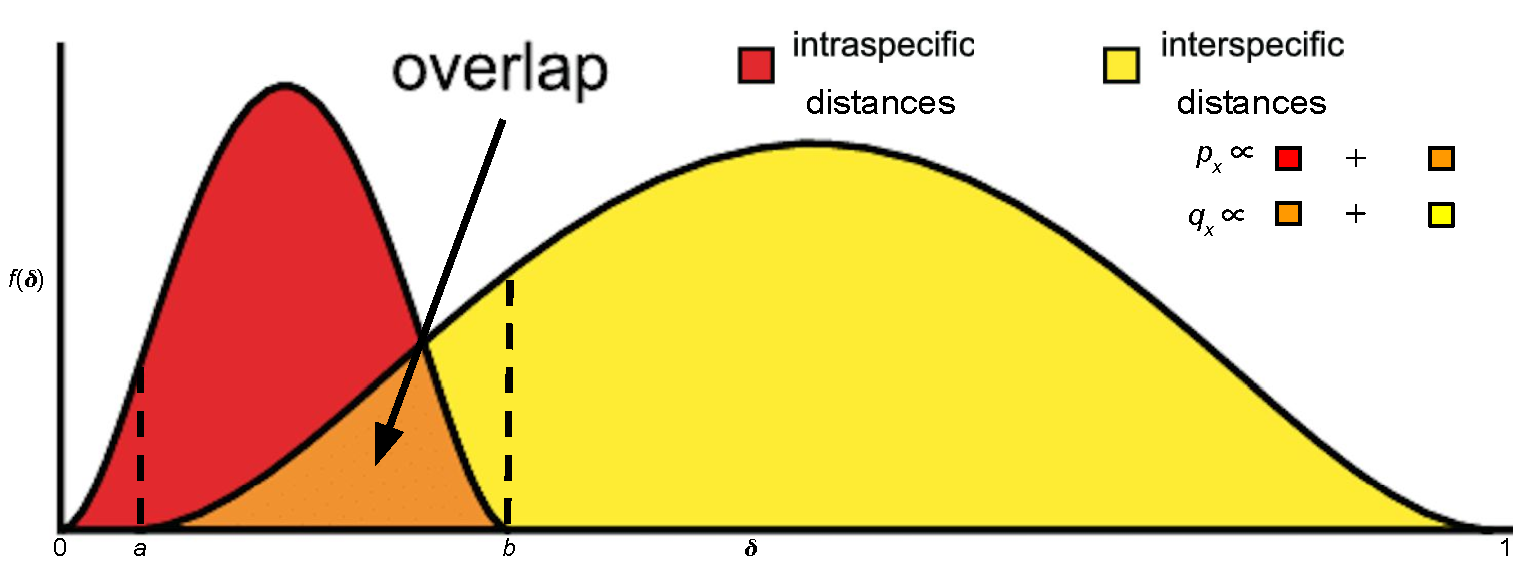
\includegraphics[width=1.0\textwidth]{Figure1}

\caption{Modified depiction from \citet{meyer2005dna} and \citet{phillips2024measure} of the overlap/separation of intraspecific and interspecific distances ($\delta$) for calculation of the DNA barcode gap metrics ($p_x$ and $q_x$) for a hypothetical species $x$. The minimum interspecific distance is denoted by $a$ and the maximum intraspecific distance is indicated by $b$. The quantity $f(\delta)$ is akin to a kernel density estimate of the probability density function of distances. A similar visualization can be displayed for $p^{'}_x$ and $q^{'}_x$ within the interval [$a'$, $b$].}

\end{figure}

\noindent Hence, Equations (1)-(4) are simply empirical partial means of distances falling at and below, or at and exceeding, given distribution thresholds. Notice further that $a$/$a'$, and $b$ are also the first and $n$th order statistics, $X_{(1)}$ and $X_{(n)}$, respectively, with  $a$/$a' < b$,  which have been pointed out by \citet{phillips2022lack} as important for developing a mathematical theory to test the existence of the DNA barcode gap. Equations (1)-(4) can also be expressed in terms of empirical cumulative distribution functions (ECDFs) (see next section). Distances form a continuous distribution and are easily computed from a model of DNA sequence evolution, such as uncorrected or corrected p-distances \citep{jukes1969evolution, kimura1980simple} using, for example, the {\tt dist.dna()} function available in the {\tt ape} R package \citep{paradis2004ape}. However, computed values are \textit{not} independent and identically distributed (IID) because estimated standard errors (SEs) will depend on both the number of species sampled with the genus under study, as well as the number of specimens sampled within a target species. In \citet{phillips2024measure}, To tease this out, \citet{phillips2024measure} suggests plotting estimator values against their estimated SEs, along with a simple random downsampling scheme. In the case of two species comprising a focal genus, one well sampled and the other poorly sampled, values of the metrics close to zero for the sufficiently sampled species will likely possess larger SEs following downsizing to match the number of poorly sampled specimens \citep{phillips2024measure}. The approach of \citet{phillips2024measure} differs markedly from the traditional definition of the DNA barcoding gap laid out by \citet{meyer2005dna} and \citet{meier2008use} in that the proposed metrics incorporate interspecific distances which \textit{include} the target species of interest. Furthermore, if a focal species is found to have multiple nearest neighbours, then the species possessing the smallest average distance is used \citep{phillips2024measure}. These schemes more accurately account for species' coalescence processes inferred from contemporaneous samples of DNA sequences leading to instances of barcode sequence sharing, such as interspecific hybridization/introgression events \citep{phillips2024measure}. Within Equations (3) and (4), the degree of distance distribution overlap between a target taxon and its nearest neighbouring species, gauged from magnitudes of $p'_x$ and $q'_x$, is directly proportional to the amount of time in which the two lineages diverged from the MRCA \citep{phillips2024measure}. Thus, the quantities can be used as a criterion to assess the failure of DNA barcoding in recently radiated taxonomic groups, among other plausible biological explanations.  Note, distances are constrained to the interval [0, 1], whereas the metrics are defined only on the interval [$a$/$a'$, $b$]. Values of the estimators obtained from Equations (1)-(4) close to or equal to zero give evidence for separation between intraspecific and interspecific distance distributions; that is, values suggest the presence of a DNA barcode gap for a target species. Conversely, values near or equal to one give evidence for distribution overlap; that is, values likely indicate the absence of a DNA barcode gap. 

\subsection{The Model}

Before delving into the derivation of the proposed DNA barcode gap metrics, review of some fundamental statistical theory is necessary.

For a given random variable $X$, its cumulative distribution function (CDF) is defined by

\begin{align}
F_X(t) = \mathbb{P}(X \leq t) = 1 - \mathbb{P}(X > t). 
\end{align}

\noindent Rearranging Equation (5) gives

\begin{align}
\mathbb{P}(X > t) = 1 - F_X(t) = 1 - \mathbb{P}(X \leq t) ,
\end{align}

\noindent from which it follows that

\begin{align}
\mathbb{P}(X \geq t) = 1 - F_X(t) + \mathbb{P}(X = t).
\end{align}

Equations (1)-(4) can thus be expressed in terms of ECDFs as follows, since the true underlying CDFs, $F(\cdot)$, are unknown \textit{a priori}, and therefore must be estimated using available data:

\begin{align}
p_x  &= \mathbb{P}(d_{ij} \geq a) \notag \\
     &= 1 - \hat{F}_{d_{ij}}(a) + \mathbb{P}(d_{ij} = a) \notag \\
     &= \hat{F}_{d_{ij}}(b) - \hat{F}_{d_{ij}}(a) +  \mathbb{P}(d_{ij} = a) \\[1ex]
q_x  &=  \mathbb{P}(d_{XY} \leq b) \notag \\
     &= \hat{F}_{d_{XY}}(b) \\[1ex]
p'_x &=  \mathbb{P}(d_{ij} \geq a') \notag \\
     &= 1 - \hat{F}_{d_{ij}}(a') +  \mathbb{P}(d_{ij} = a') \notag \\
     &= \hat{F}_{d_{ij}}(b) - \hat{F}_{d_{ij}}(a') +  \mathbb{P}(d_{ij} = a')  \\[1ex]
q'_x &=  \mathbb{P}(d'_{XY} \leq b) \notag \\
     &= \hat{F}_{d'_{XY}}(b)
\end{align}

\noindent From this, it can be seen that $\hat{F}_{d_{ij}}(b) = 1$ in Equations (8) and (10). Given $n$ \\ increasing-ordered data points, the (discrete) ECDF, $\hat{F}_n(t) = \frac{1}{n}\sum_{i = 1}^n\mathds{1}_{[x_i \leq t]}$, comprises a step function having jump discontinuities of size $\frac{1}{n}$ at each sample observation ($x_i$), excluding ties (or steps of weight $\frac{i}{n}$ with duplicate observations), where $\mathds{1}(x)$ is the indicator function. Note, $\mathbb{P}(X = t) \neq 0$. Equations (8)-(11) clearly demonstrate the asymmetric directionality of the proposed metrics. Furthermore, calculation of the DNA barcode gap estimators is convenient as they implicitly account for total distribution area (including overlap).

A major criticism of large sample (frequentist) theory is that it relies on asymptotic properties of the MLE (whose population parameter is assumed to be a fixed but unknown quantity), such as estimator normality and consistency as the sample size approaches infinity. This problem is especially pronounced in the case of binomial proportions \citep{newcombe1998confidence}. The estimated Wald SE of the sample proportion, is given by $\widehat{SE[\hat{p}}] = \sqrt{\frac{\hat{p}(1 - \hat{p})}{n}}$, where $\hat{p} = \frac{Y}{n}$ is the MLE, $Y$ is the total number of successes ($Y = \sum_{i=1}^n{y_i}$), and $n$ is the total number of trials (\textit{i.e.}, sample size). However, the above formula for the standard error is problematic for several reasons. First, it is a Normal approximation which makes use of the central limit theorem (CLT); thus, large sample sizes are required for reliable estimation. When few observations are available, SEs will be large and inaccurate, leading to low statistical power to detect a true DNA barcode gap when one actually exists. Further, resulting interval estimates could span values less than zero or greater than one, or have zero width, which is practically meaningless. Second, when proportions are exactly equal to zero or one, resulting SEs will be exactly zero, rendering $\widehat{SE[\hat{p}}]$ given above completely useless. In the context of the proposed DNA barcode gap metrics, values obtained at the boundaries of their support are often encountered. Therefore, reliable calculation of SEs is not feasible. Given the importance of sufficient sampling of species genetic diversity for DNA barcoding initiatives, a different statistical estimation approach is necessary. 

Bayesian inference offers a natural path forward in this regard since it allows for \\ straightforward specification of prior beliefs concerning unknown model parameters and permits the seamless propagation of uncertainty, when data are lacking and sample sizes are small, through integration with the likelihood function associated with true generating processes. The posterior distribution ($\pi(\theta | Y)$) is given by Bayes' theorem up to a \\ proportionality $\pi(\theta | Y) \propto \pi(Y | \theta)\pi(\theta)$, where $\theta$ are unobserved parameters, $Y$ are known data, $\pi(Y | \theta)$ is the likelihood, and $\pi(\theta)$ is the prior.  As a consequence, because parameters are treated as random variables, Bayesian models are much more flexible and generally more easily interpretable compared to frequentist approaches. Under the Bayesian paradigm, entire posterior distributions, along with their summaries (\textit{e.g.}, CrIs) are outputted, rather than just long run behaviour reflected in sampling distributions, p-values, and CIs as in the frequentist case, thus allowing direct probability statements to be made. 

Essentially, from a statistical perspective, the goal herein is to nonparametrically estimate probabilities corresponding to extreme tail quantiles for positive highly skewed distributions on the unit interval  (or any closed subinterval thereof). Here, it is sought to numerically approximate the extent of proportional overlap/separation of intraspecific and interspecific distance distributions within the subinterval [$a/a'$, $b$]. This is a challenging computational problem within the current study as detailed in subsequent sections. The usual approach employs kernel density estimation (KDE), along with numerical or Monte Carlo integration of complicated probability distribution functions (PDFs), and invocation of extreme value theory (EVT); however, this requires careful selection of the bandwidth parameter, among other considerations. This becomes problematic when fitting finite mixture models where nonidentifiability is rampant. For DNA barcode gap estimation, this would correspond to a two-component mixture (one for intraspecific distance comparisons, and the other for interspecific comparisons), with one or more curve intersection points between components, and the presence of zero distance inflation. This makes parameter estimation difficult using methods like the Expectation-Maximization (EM) algorithm \citep{dempster1977maximum} as the algorithm may become stuck in suboptimal regions of the parameter search space and prematurely converge to local optima. Here, for simplicity, an alternate route is taken to avoid these obstacles. Counts, $y$, of overlapping distances (as expressed in the numerator of Equations (1)-(4)) are treated as binomially distributed with expectation $\mathbb{E}[Y] = k\theta$, and variance $\mathbb{V}[Y] = k\theta(1 - \theta)$, where $k = \{N, C\}$ are total count vectors of intraspecific and combined interspecific distances, respectively, for a target species along with its nearest neighbour species, and $k = M$ is a total count vector for all interspecific species comparisons. This follows from the fact that the ECDF is binomially distributed. The quantity thus being estimated is the parameter vector $\underaccent{\bar}{\theta} = \{p_x, q_x, p^{'}_x, q^{'}_x\}$. 

The metrics encompassing $\underaccent{\bar}{\theta} $ are presumed to follow a Beta($\alpha$, $\beta$) distribution, with real shape parameters $\alpha$ and $\beta$, which is a natural choice of prior on probabilities. The beta distribution has a prior mean of $\mathbb{E}[\theta] = \frac{\alpha}{\alpha + \beta}$ and a prior variance equal to $\mathbb{V}[\theta] = \frac{\alpha\beta}{(\alpha + \beta)^2(\alpha + \beta + 1)}$. In the case where $\alpha = \beta$, all generated Beta($\alpha$, $\beta$) distributions will possess the same prior expectation, whereas the prior variance will shrink as both $\alpha$ and $\beta$ increase. Such a scheme is quite convenient since the beta distribution is conjugate to the binomial distribution. Thus, the posterior distribution is also beta distributed, specifically, Beta($\alpha + Y$, $\beta + n - Y$), having expectation $\mathbb{E}[\theta|Y] = \frac{\alpha + Y}{\alpha + \beta + n}$ and variance $\mathbb{V}[\theta|Y] = \frac{(\alpha + Y)(\beta + n - Y)}{(\alpha + \beta + n)^2(\alpha + \beta + n + 1)}$. In the context of DNA barcoding, it is important that the DNA barcode gap metrics effectively differentiate between extremes of no overlap/complete separation and complete overlap/no separation, corresponding to values of the metrics equal to 0 and 1 (equivalent to total distance counts of 0 and $n$), respectively. These extremes yield a posterior expectation of\\  $\mathbb{E}[\theta|Y = 0] = \frac{\alpha}{\alpha + \beta + n}$ and a posterior variance of $\mathbb{V}[\theta|Y = 0] = \frac{\alpha(\beta + n)}{(\alpha + \beta + n)^2(\alpha + \beta + n + 1)}$ and \\ $\mathbb{E}[\theta|Y = n] = \frac{\alpha + n}{\alpha + \beta + n}$ and $\mathbb{V}[\theta|Y = n] = \frac{(\alpha + n)\beta}{(\alpha + \beta + n)^2(\alpha + \beta + n + 1)}$. Note, the posterior variances are equivalent at these thresholds for all $\alpha$ = $\beta$.

Parameters were given an uninformative Beta(1, 1) prior, which is equivalent to a standard uniform (Uniform(0, 1)) prior since it places equal probability on all parameter values within its support. This distribution has an expected value of $\mu = \frac{1}{2}$ = 0.500 and a variance of $\sigma^2 = \frac{1}{12} \approx 0.083$. Further, the posterior is Beta($Y + 1$, $n - Y + 1$), from which various moments such as the expected value $\mathbb{E}[\theta|Y] = \frac{Y + 1}{n + 2}$ and variance $\mathbb{V|\theta}[Y] = \frac{(Y + 1)(n - Y + 1)}{(n + 2)^2(n + 3)}$, and other quantities, can be easily calculated. Clearly, $\mathbb{E}[\theta|Y = 0] = \frac{1}{n + 2}$ and $\mathbb{V}[\theta|Y = 0] = \frac{n + 1}{(n + 2)^2(n + 3)}$, and $\mathbb{E}[\theta|Y = n] = \frac{n + 1}{n + 2}$ and $\mathbb{V}[\theta|Y = n] = \frac{n + 1}{(n + 2)^2(n + 3)}$. For example, with $n$ = 2 sampled specimens for a given species (the minimum sample size possible) having no overlapping genetic distances, on average, $\theta$ will be equal to $\mu = \frac{1}{4}$ = 0.250, with a variance of \\ $\sigma^2 = \frac{3}{80} \approx$ 0.0375. In contrast, with $n$ = 100 and no overlap, the mean reduces to \\ $\mu = \frac{1}{102} \approx$ 0.001, with a variance of $\sigma^2$ = 9.425$\hspace{1mm} \times \hspace{1mm} 10^{-5}$. When $n$ = 2 and both taxon distances overlap, the mean is $\mu = \frac{3}{4}$ = 0.750, having a variance of $\sigma^2 \approx$ 0.0375. For $n$ = 100 where all distances overlap, $\theta$ has expectation $\mu = \frac{101}{102} \approx$ 0.990 and variance $\sigma^2 \approx$ 9.425$\hspace{1mm} \times \hspace{1mm} 10^{-5}$. These edge case examples demonstrate that the Beta(1, 1) distribution serves as a good first-pass prior for DNA barcode gap estimation using \citeauthor{phillips2024measure}'s (\citeyear{phillips2024measure}) metrics, though tighter bounds can still be achieved. In general however, when possible, it is always advisable to incorporate prior information, even if only weak, rather than simply imposing complete ignorance in the form of a flat prior distribution. In the case of unimodal distributions, the (estimated) posterior mean often possesses the property that it readily decomposes into a convex linear combination, in the form of a weighted sum, of the (estimated) prior mean and the MLE. That is $\hat{\mu}_\mathrm{posterior} = w\hat{\mu}_\mathrm{prior} + (1-w)\hat{\mu}_\mathrm{MLE}$, where for the beta distribution, $w = \frac{\alpha + \beta}{\alpha + \beta + n}$. Therefore, with sufficient data, $w \rightarrow 0$ as $n \rightarrow \infty$, regardless of the values of $\alpha$ and $\beta$, and the choice of prior distribution becomes less important since the posterior will be dominated by the likelihood. For the Beta(1, 1), $w = \frac{2}{2 + n}$, with $n$ = 2 giving $w = \frac{1}{2}$ = 0.500; that is, the posterior is the arithmetic average of the prior and the likelihood. For $n$ = 100, the prior weight is $w = \frac{2}{102} \approx$ 0.0196. The full Bayesian model for species $x$ is thus given by

\begin{align}
\notag y_\mathrm{lwr} &\sim \mathrm{Binomial}(N, p_\mathrm{lwr}) \\ 
\notag y_\mathrm{upr} &\sim \mathrm{Binomial}(M, p_\mathrm{upr}) \\ 
y^{'}_\mathrm{lwr} &\sim \mathrm{Binomial}(N, p^{'}_\mathrm{lwr}) \\ 
 \notag y^{'}_\mathrm{upr} &\sim \mathrm{Binomial}(C, p^{'}_\mathrm{upr}) \\ 
\notag p_\mathrm{lwr}, p_\mathrm{upr}, p^{'}_\mathrm{lwr}, p^{'}_\mathrm{upr}
&\sim \mathrm{Beta}(1, 1).
\end{align}

\noindent Note that $p_x$, $q_x$, $p^{'}_x$, and $q^{'}_x$ in Equations (1)-(4) are denoted $p_\mathrm{lwr}$, $p_\mathrm{upr}$, $p^{'}_\mathrm{lwr}$, $q^{'}_\mathrm{upr}$ within Equation (12) for easy distinction between MLEs and Bayesian posterior estimates. The above statistical theory and derivations lay a good foundation for the remainder of this paper.

The proposed model is inherently vectorized to allow processing of multiple species datasets simultaneously. Model fitting was achieved using the Stan probabilistic \\ programming language \citep{carpenter2017stan} framework for Hamiltonian Monte Carlo (HMC) via the No-U-Turn Sampler (NUTS) sampling algorithm \citep{hoffman2014no} through the {\tt rstan} R package (version 2.32.6) \citep{stan2023rstan} in R (version 4.4.1) \citep{rcore2024language}. Four Markov chains were run for 2000 iterations each in parallel across four cores with random parameter initializations. Within each chain, a total of 1000 samples was discarded as warmup (\textit{i.e.}, burnin) to reduce dependence on starting conditions and to ensure posterior samples are reflective of the equilibrium distribution. Further, 1000 post-warmup draws were utilized per chain during the sampling phase. Because HMC/NUTS results in dependent samples that are minimally autocorrelated, chain thinning is not required. Each of these tuning parameters reflect default Markov Chain Monte Carlo (MCMC) settings in Stan to control both bias and variance respectively in the resulting draws. All analyses in the present work were carried out on a 2023 Apple MacBook Pro with M2 chip and 16 GB RAM running macOS Ventura 13.2. A random seed was set to ensure reproducibility of model results. Outputted estimates were rounded to three decimal places of precision. Posterior distributions were visualized as KDE plots using the {\tt ggplot2} R package (version 3.5.1) \citep{wickham2016ggplot2} with the default Gaussian kernel and optimal smoothness selection. To successfully run the Stan program, end users must have installed an appropriate compiler (such as GCC or Clang) which is compatible with their operating system, such as macOS.

Convergence was assessed both visually and quantitatively as follows: (1) through \\ examining parameter traceplots, which depict the trajectory of accepted MCMC draws as a function of the number of iterations, (2) through monitoring the Gelman-Rubin potential scale reduction factor statistic   ($\hat{R}$)  \citep{gelman1992iterative, vehtari2017rank}, which measures the concordance of within-chain \textit{versus} between-chain variance, and (3) through calculating the effective sample size (ESS) for each parameter, which quantifies the number of independent samples generated Markov chains are equivalent to. Mixing of chains was deemed sufficient when traceplots looked like ``fuzzy caterpillars", $\hat{R} < 1.01$, and effective sample sizes were reasonably large \citep{gelman2020bayesian}.
After sampling, a number of summary quantities were reported, including posterior means, posterior SDs, and posterior quantiles from which 95\% CrIs could be computed to make probabilistic inferences concerning true population parameters. To validate the overall correctness of the proposed statistical model given by Equation (12), as a means of comparison, posterior predictive checks (PPCs) were also employed to generate binomial random variates in the form of counts from the posterior predictive distribution; that is $\underaccent{\bar}{\gamma} = \{Np_x, Mq_x, Np^{'}_x, Cq^{'}_x\}$ to verify that the model adequately captures relevant features of the observed data. The proposed Bayesian model outlined here has a straightforward interpretation (\textbf{Table 1}). 

\begin{table}[htbp]
    \centering
    \small
    \caption{Interpretation of the DNA barcode gap estimators within [$a/a'$, $b$]}.
    \label{tab:parameters}
    \begin{tabular}{cp{0.7\linewidth}}
    \hline
    \textbf{Parameter} & \textbf{Explanation} \\
    \hline
    $p_x$/$p_{\text{lwr}}$ & When $p_{\text{lwr}}$ is close to 0 (1), it suggests that the probability of intraspecific (interspecific) distances being larger (smaller) than interspecific (intraspecific) distances is low (high) on average, while the probability of interspecific (intraspecific) distances being larger (smaller)  than intraspecific (interspecific) distances is high (low) on average; that is, there is (no) evidence for a DNA barcode gap.\\
        & \\[-2mm]
     $q_x$/$p_{\text{upr}}$ & When $p_{\text{upr}}$ is close to 0 (1), it suggests that the probability of interspecific (intraspecific) distances being larger (smaller) than intraspecific (interspecific) distances is high (low) on average, while the probability of intraspecific (interspecific) distances being larger (smaller) than interspecific (intraspecific) distances is low (high) on average; that is, there is (no) evidence for a DNA barcode gap. \\
        & \\[-2mm]
    $p^{'}_x$/$p^{'}_{\text{lwr}}$ & When $p^{'}_{\text{lwr}}$ is close to 0 (1), it suggests that the probability of intraspecific (combined interspecific distances for a target species and its nearest neighbour species) distances being larger than combined interspecific distances for a target species and its nearest neighbour species (intraspecific distances) is low (high) on average, while the probability of combined interspecific distances for a target species and its nearest neighbour species (intraspecific distances) being larger than intraspecific distances (combined interspecific distances for a target species and its nearest neighbour species) is high (low) on average; that is, there is (no) evidence for a DNA barcode gap.\\
        & \\[-2mm]
     $q^{'}_x$/$p^{'}_{\text{upr}}$ & When $p^{'}_{\text{upr}}$ is close to 0 (1), it suggests that the probability of combined interspecific distances for a target species and its nearest neighbour species (intraspecific distances) being larger than intraspecific distances (combined interspecific distances for a target species and its nearest neighbour species) is high (low) on average, while the probability of intraspecific distances (combined interspecific distances for a target species and its nearest neighbour species) being larger than combined interspecific distances for a target species and its nearest neighbour species (intraspecific distances) is low (high) on average; that is, there is (no) evidence for a DNA barcode gap.\\
    \hline
    \end{tabular}
\end{table}

\section{Results and Discussion}

The \textit{Agabus} CYTB dataset analyzed by \citet{phillips2024measure} is revisited herein for the species \textit{A. bipustulatus} and \textit{A. nevadensis}, since these taxa were the sole representatives for this locus, with the most and the least specimen records, respectively ($N$ = 701 and \\ $N$ = 2) across all three assessed molecular markers. Briefly, using the R package {\tt MACER} \citep{young2021macer}, DNA sequences were downloaded from GenBank and BOLD and processed to obtain a 343 bp FASTA alignment representing 46 unique haplotypes. Genetic distances were calculated using uncorrected p-distances. Further, \textit{A. bipustulatus} comprised 46 total haplotypes, whereas \textit{A. nevadensis} possessed two haplotypes. Note, DNA barcode gap estimation is only possible for species having at least two specimen records. This dataset is a prime illustrative example highlighting the issue of inadequate taxon sampling, which arises frequently in large-scale phylogenetic and phylogeographic studies, in several respects. First, from a statistical viewpoint, sample sizes reflect extremes in reliable parameter \\ estimation. Second, from a DNA barcoding perspective, \textit{Agabus} currently comprises about 200 extant species according to the Global Biodiversity Information Facility (GBIF) \\ (https://www.gbif.org); yet, due to the level of convenience sampling inherent in taxonomic collection efforts for this genus, adequate representation of species and genetic diversity is far from complete. 

MCMC parameter traceplots showed rapid mixing of chains to the stationary distribution (\textbf{Supplementary Figure 1}). Further, all $\hat{R}$ and ESS values (not shown) were close to their recommended cutoffs of one and thousands of samples, respectively, indicating chains are both well-mixed and have converged to the posterior distribution.  

Bayesian posterior estimates were reported alongside frequentist MLEs, in addition to SEs, posterior SDs, 95\% CIs and 95\% CrIs (\textbf{Table 2}).

\begin{table}[H]

\small

\centering

\caption{Nonparametric frequentist and Bayesian estimates of distance distribution overlap/separation for the DNA barcode gap coalescent model parameters applied to \textit{A. bipustulatus} ($N$ = 701) and \textit{A. nevadensis} ($N$ = 2) for CYTB, including 95\%  CIs and CrIs. CrIs are based on 4000 posterior draws. All parameter estimates are reported to three decimal places of precision.}

\begin{tabular}{cccc} \hline

\textbf{Species} & \textbf{Parameter} & \textbf{MLE (SE, 95\% CI)} & \textbf{Bayes Est. (SD; 95\% CrI)} \\  \hline
\textit{A. bipustulatus} & $p_x/p_\mathrm{lwr}$ & 1.000 (0.000; 1.000-1.000) & 1.000 (0.000; 1.000-1.000) \\
\textit{A. bipustulatus} & $q_x/p_\mathrm{upr}$ & 1.000 (0.000; 1.000-1.000) & 1.000 (0.000; 0.999-1.000) \\
\textit{A. bipustulatus} & $p^{'}_x/p^{'}_\mathrm{lwr}$ & 1.000 (0.000; 1.000-1.000) & 1.000 (0.000; 1.000-1.000)  \\
\textit{A. bipustulatus} & $q^{'}_x/p^{'}_\mathrm{upr}$ & 1.000 (0.000; 1.000-1.000) & 1.000 (0.000; 0.999-1.000) \\


\textit{A. nevadensis} & $p_x/p_\mathrm{lwr}$ & 1.000 (0.000; 1.000-1.000) & 0.835 (0.144; 0.470-0.996) \\
\textit{A. nevadensis} & $q_x/p_\mathrm{upr}$ & 0.010 (0.002; 0.006-0.014) & 0.010 (0.002; 0.007-0.014) \\
\textit{A. nevadensis} &  $p^{'}_x/p^{'}_\mathrm{lwr}$ & 1.000 (0.000; 1.000-1.000) & 0.834 (0.138; 0.481-0.994) \\
\textit{A. nevadensis} &  $q^{'}_x/p^{'}_\mathrm{upr}$ & 0.010 (0.070; -0.128-0.148) & 0.010 (0.002; 0.007-0.014) \\


\hline


\end{tabular}

\end{table}


\noindent  CIs were calculated using the usual large sample  $(1-\alpha)100\%$-level interval estimate given by $\hat{p} \hspace{1mm} \pm z_{1 - \frac{\alpha}{2}}\sqrt{\frac{\hat{p}(1 - \hat{p})}{n}}$, where $z_{1 - \frac{\alpha}{2}}$ = 1.960 is the critical value for 95\% confidence (\textit{i.e.}, the 97.5th percent quantile from the standard Normal distribution), and $\alpha$ is the stated significance level (here, 5\%). Given a ($1 - \alpha$)100\% CI, with repeated sampling, on average ($1 - \alpha$)100\% of constructed intervals will contain the true parameter of interest, assuming a correctly specified statistical model; on the other hand, any given CI will either capture or exclude the true parameter with 100\% certainty. This in stark contrast to a CrI, where the true parameter is contained within said interval with ($1 - \alpha$)100\% probability, contingent on the data generating model being correct. Note, by default Stan computes equal-tailed (central) CrIs such that there is equal area situated in the left and right tails of the posterior distribution. For a 95\% CrI, this corresponds to the 2.5th and 97.5th percent quantiles. However, constructed intervals are usually only valid for symmetric or nearly symmetric distributions. Given the bounded nature of the DNA barcode gap metrics, whose posterior distributions, as expected, show considerable skewness, an alternative approach to reporting CrIs, such as Highest Posterior Density (HPD) intervals \citep{chen1999monte} or shortest probability intervals (SPIn) \citep{liu2015simulation} is warranted. As such asymmetric intervals generally attain greater statistical efficiency (in the form of smaller Mean Squared Error (MSE) or variance) and higher coverage probabilities than more standard interval estimates, careful in-depth comparison is left for future work. 

Findings based on nonparametric MLEs and Bayesian posterior means were quite \\ comparable with one another and show evidence of complete overlap in intraspecific, \\ interspecific, and combined interspecific distances for \textit{A. bipustulatus} in both the \\ $p$/$q$/$p_{\mathrm{lwr}}$/$p_{\mathrm{upr}}$ and $p'$/$q'$/$p^{'}_{\mathrm{lwr}}$/$p^{'}_{\mathrm{upr}}$ directions since the metrics attain magnitudes very close to one, with minimsl noise (\textbf{Table 2}). As a result, this likely indicates that no DNA barcode gap is present for this species. Such findings are strongly reinforced by the very tight clustering of posterior draws (\textbf{Figure 2}) and associated interval estimates owing to the large number of specimens sampled for this species.

\begin{figure}[H]

\centering

\small

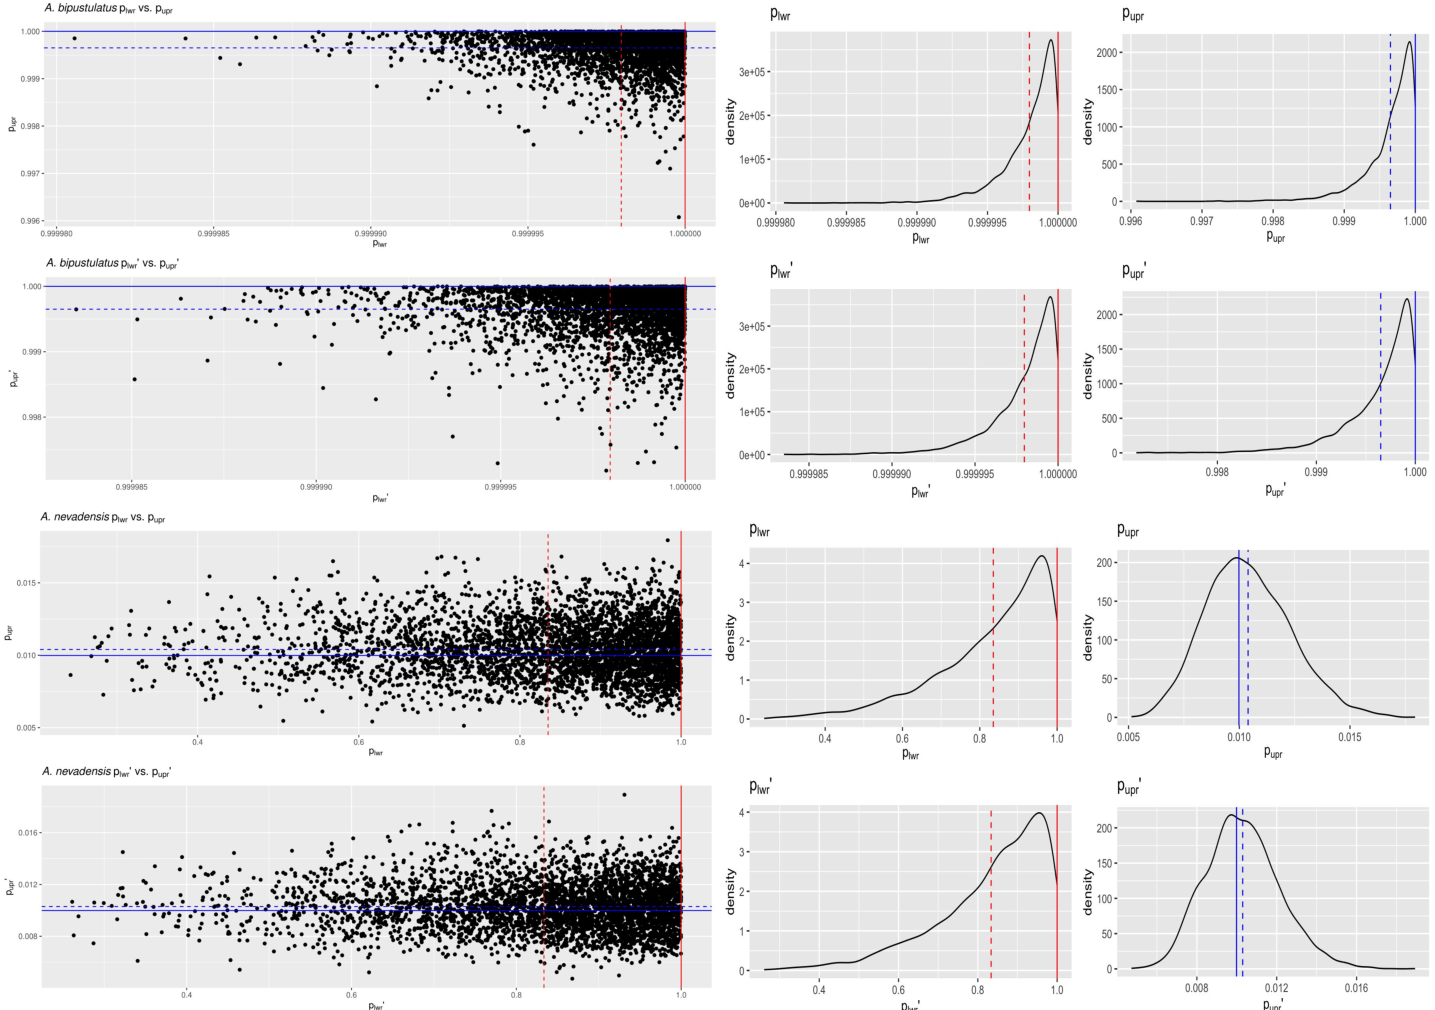
\includegraphics[width=0.80\textwidth]{Figure2}

\caption{Scatterplots (black solid points) and distributions (black solid lines) depicting the DNA barcode gap metrics for \textit{A. bipustulatus} ($N$ = 701) and  \textit{A. nevadensis} ($N$ = 2) across CYTB based on 4000 Bayesian posterior draws. MLEs and posterior means are displayed as coloured (red/blue) solid and dashed lines for the metrics, respectively.}

\end{figure}

\noindent On the other hand, the situation for \textit{A. nevadensis} is more nuanced, as posterior values are further spread out (\textbf{Table 2} and \textbf{Figure 2}), suggesting less overall certainty in true parameter values given the low specimen sampling coverage for this taxon. Of note, calculated SEs and SDs are large, with the 95\% CIs and 95\% CrIs being quite wide in most cases, consistent with much uncertainty regarding the computed frequentist and Bayesian posterior means of the DNA barcode gap metrics. For instance, the Bayesian analysis suggests that the data are consistent with both $p_{\mathrm{lwr}}$ and $p^{'}_{\mathrm{lwr}}$ ranging from approximately 0.500-1.000 due to the large SD of about 0.140. The posterior means associated with these estimates themselves are also far from one. The CrI for $p_{\mathrm{upr}}$ and $p^{'}_{\mathrm{upr}}$ also spans an order of magnitude. Further, regarding the frequentist analysis for the same species, the 95\% CI for $q_x$ is quite wide, reflecting considerable uncertainty in its true parameter value. Similarly, that for $q^{'}_x$ extends to negative values at the left endpoint, due to the corresponding SE of 0.070 being too high as a result of the extremely low sample size of $n$ = 2 individuals sampled (\textbf{Table 2}). Since the 95\% CI for $q^{'}_x$ truncated at the lower endpoint includes the value of zero, the null hypothesis for the presence of a DNA barcode gap cannot be rejected. Despite this, it is worth noting that truncation is not standard statistical practice and will likely lead to an interval with less than 95\% nominal coverage. In such cases, more appropriate confidence interval methods like the Wilson score interval, the exact (Clopper-Pearson) interval, or the Agresti-Coull interval should be employed \citep{newcombe1998confidence, agresti1998approximate}. KDEs for \textit{A. bipustulatus} are strongly left (negatively) skewed (\textbf{Figure 2}), whereas those for \textit{A. nevadensis} exhibit more symmetry, especially for $p_{\mathrm{upr}}$ and $p^{'}_{\mathrm{upr}}$ (\textbf{Figure 2}). These differences are likely due to the stark contrast in sample sizes for the two examined species. Nevertheless, simulated counts of overlapping specimen records from the posterior predictive distribution (\textbf{Supplementary Table 1}) were found to be very close to observed counts for both species, indicating that the proposed model adequately captures underlying variation. Obtained results suggest that use of the Beta(1, 1) prior may not be appropriate given a low number of collected individuals for most taxa in DNA barcoding efforts. This suggests that further consideration of more informative beta priors is worthwhile. This is clear for \textit{A. nevadensis}, where use of a stronger prior will likely eliminate the issue regarding accurate estimation of $p_{\mathrm{lwr}}$ and $p^{'}_{\mathrm{lwr}}$ and stabilize their uncertainty.

\section{Conclusion}

Herein, the accuracy of the DNA barcode gap was analyzed from a rigorous statistical lens to expedite both the curation and growth of reference sequence libraries, ensuring they are populated with high quality, statistically defensible specimen records fit for purpose to address standing questions in ecology, evolutionary biology, management, and conservation. To accomplish this, recently proposed, easy to calculate nonparametric MLEs were formally derived using ECDFs and applied to assess the extent of overlap/separation of distance distributions within and among two species of predatory water beetles in the genus \textit{Agabus} sequenced at CYTB using a Bayesian binomial count model with conjugate beta priors. Findings highlight a high level of parameter uncertainty for \textit{A. nevadensis}, whereas posterior estimates of the DNA barcode gap metrics for \textit{A. bipustulatus} are much more certain. Based on these results, it is imperative that specimen sampling be prioritized to better reflect actual species boundaries. More generally, apart from the metrics being employed to better highlighting the importance of within-species genetic diversity versus between-species divergence, it is expected that the approach developed herein will be of broad utility in applied fields, such as DNA-based detection of seafood fraud within global supply chains, and in the determination of species occupancy/detection probabilities at ecological sites of interest using active and passive environmental DNA (eDNA) methods such as metabarcoding.

Since the DNA barcode gap metrics often attain values very close to zero (suggesting no overlap and complete separation of distance distributions) and/or very near one (indicating no separation and complete overlap), in addition to more intermediate values, a noninformative Beta($\frac{1}{2}, \frac{1}{2}$) prior may be more appropriate over complete ignorance imposed by a Beta(1, 1) prior. The former distribution is U-shaped symmetric and places greater probability density at the extremes of the distribution due to its heavier tails, while still allowing for variability in parameter estimates within intermediate values along its domain. Note that this prior is Jeffreys' prior density \citep{jeffreys1946invariant}, which is  proportional to the square root of the Fisher information $\mathcal{I}(\theta)$; that is,
$\pi(\theta) \propto \theta^{-\frac{1}{2}}(1-\theta)^{-\frac{1}{2}}$. Jeffreys' prior has several desirable statistical  properties as a prior: that it is inversely proportional to the standard deviation of the binomial distribution, and most notably, that it is invariant to model reparameterization \citep{gelman2014bayesian}. However, this prior can lead to divergent transitions, among other pathologies, imposed by complex geometry (\textit{i.e.}, curvature) in the posterior space since many iterative stochastic MCMC sampling algorithms experience difficulties when exploring high density distribution regions. Thus, remedies to resolve them, such as lowering the step size of the HMC/NUTS sampler, should be attempted in future work, along with other approaches such as empirical Bayes estimation to approximate beta prior hyperparameters from observed data through the MLE or other methods of parameter estimation, such as the method of moments. Alternatively, hierarchical modelling could be employed to estimate separate distribution model hyperparameters for each species and/or compute distinct estimates for the directionality/comparison level of the DNA barcode gap metrics (\textit{i.e.,} lower \textit{vs.} upper, non-prime \textit{vs.} prime) separately within the genus under study. This would permit greater flexibility through incorporating more fine-grained structure seen in the data; however, low taxon sample sizes may preclude valid inferences to be reasonably ascertained due to the large number additional parameters which would be introduced through the specification of the hyperprior distributions. Methods outlined in \citet{gelman2014bayesian}, such as dealing with non-exchangeability of observations and alternate model parameterizations like the logit, may prove useful in this regard. Perhaps, the best course of action though is the elicitation of priors from domain experts. Even though more work remains, it is clear that both frequentist and Bayesian inference hold much promise for the future of molecular biodiversity science.


\newpage

\section*{Supplementary Information}

None declared.

\section*{Data Availability Statement}

Raw data, R, and Stan code can be accessed via Dryad at: \\ \href{http://datadryad.org/stash/share/RZIfMixcEODe0RWP7eyXWQewSVbqEIA9UTrH3ZVKyn4}{http://datadryad.org/stash/share/\\RZIfMixcEODe0RWP7eyXWQewSVbqEIA9UTrH3ZVKyn4}.

A GitHub repository can be found at: \\ \href{https://github.com/jphill01/Bayesian-DNA-Barcode-Gap-Coalescent}{https://github.com/jphill01/Bayesian-DNA-Barcode-Gap-Coalescent}.

\section*{Acknowledgements}

We wish to recognise the valuable comments and discussions of Daniel (Dan) Gillis, Robert (Bob) Hanner, Robert (Rob) Young, and XXX anonymous reviewers.

We acknowledge that the University of Guelph resides on the ancestral lands of the Attawandaron people and the treaty lands and territory of the Mississaugas of the Credit. We recognize the significance of the Dish with One Spoon Covenant to this land and offer our respect to our Anishinaabe, Haudenosaunee and M{\'e}tis neighbours as we strive to strengthen our relationships with them.

\section*{Funding}

None declared.

\section*{Conflict of Interest}

None declared.

\section*{Author Contributions}

JDP wrote the manuscript, wrote R and Stan code, as well as analyzed and interpreted all model results. 

\bibliographystyle{humannat}
\bibliography{References}

\newpage

\end{document}